% © Copyright 2011 Joachim Breitner
% Distributed under the terms of the Creative Commons Attribution license.
\documentclass{beamer}

\newcommand{\hide}{\onslide+<+(1)->}

\usetheme[titlepage0,22pt]{KIT}
\setbeamercolor{structure}{fg=KITgreen}


\usepackage[utf8]{inputenc}
\usepackage[TS1,T1]{fontenc}
\usepackage[english]{babel}
\usepackage{listings}
\usepackage{xcolor}
\usepackage{tikz}
\usetikzlibrary{backgrounds,decorations.pathreplacing}
\usepackage{mathpartir}
\usepackage{adjustbox}
\usepackage{amsmath}
\usepackage{mathtools}
\usepackage[safe]{tipa} % for \textlambda
\usepackage{wasysym}
\usepackage{stmaryrd}

\definecolor{light-gray}{gray}{0.95}
\lstdefinestyle{haskell}{
        ,columns=flexible
        ,basewidth={.365em}
        ,keepspaces=True
        ,belowskip=0pt
        ,backgroundcolor=\color{light-gray}
        ,frame=single
        ,xleftmargin=2em
        ,xrightmargin=2em
        ,basicstyle=\small\sffamily
        ,stringstyle=\itshape
        ,language=Haskell
        ,texcl=true
        ,showstringspaces=false
        ,keywords={module,where,import,data,let,in,case,of}
}
\lstnewenvironment{haskell}{\lstset{style=haskell}}{}


\title{A Haskell Roadshow}
\KITtitleimage[viewport=0 40 400 100]{screenshot}
\logo{
\includegraphics{Telekom}}
\author{Joachim Breitner}
\date{2012-12-18}
\subtitle[\insertauthor]{\insertauthor\\The Karlsruhe Functional Programmers Meetup Group\\December 18, 2012}
\iflanguage{ngerman}{%
  \institute{LEHRSTUHL PROGRAMMIERPARADIGMEN}%
}{%
  \institute{PROGRAMMING PARADIGMS GROUP}%
}


\DeclareTextSymbol\textlambda{T3}{171}           % Lambda
\DeclareTextSymbolDefault\textlambda{T3}
\DeclareUnicodeCharacter{03BB}{\textlambda}


\begin{document}

\frame[plain]{\titlepage}
\only<article>{\maketitle}

\section{Features}
\only<presentation>{\subsection*{}}

\begin{frame}
\frametitle{Haskell is know for}

being a
\begin{center}
\Large
functional\\pure\\lazy evaluated\\strongly typed\\interpreted\\compiled
\end{center}
programming language \ldots

\raggedleft
\pause
and it is \alert{fun} to program in.

\end{frame}

\begin{frame}
\frametitle{Lets demonstrate that}

Visualize (one aspect) of this data:

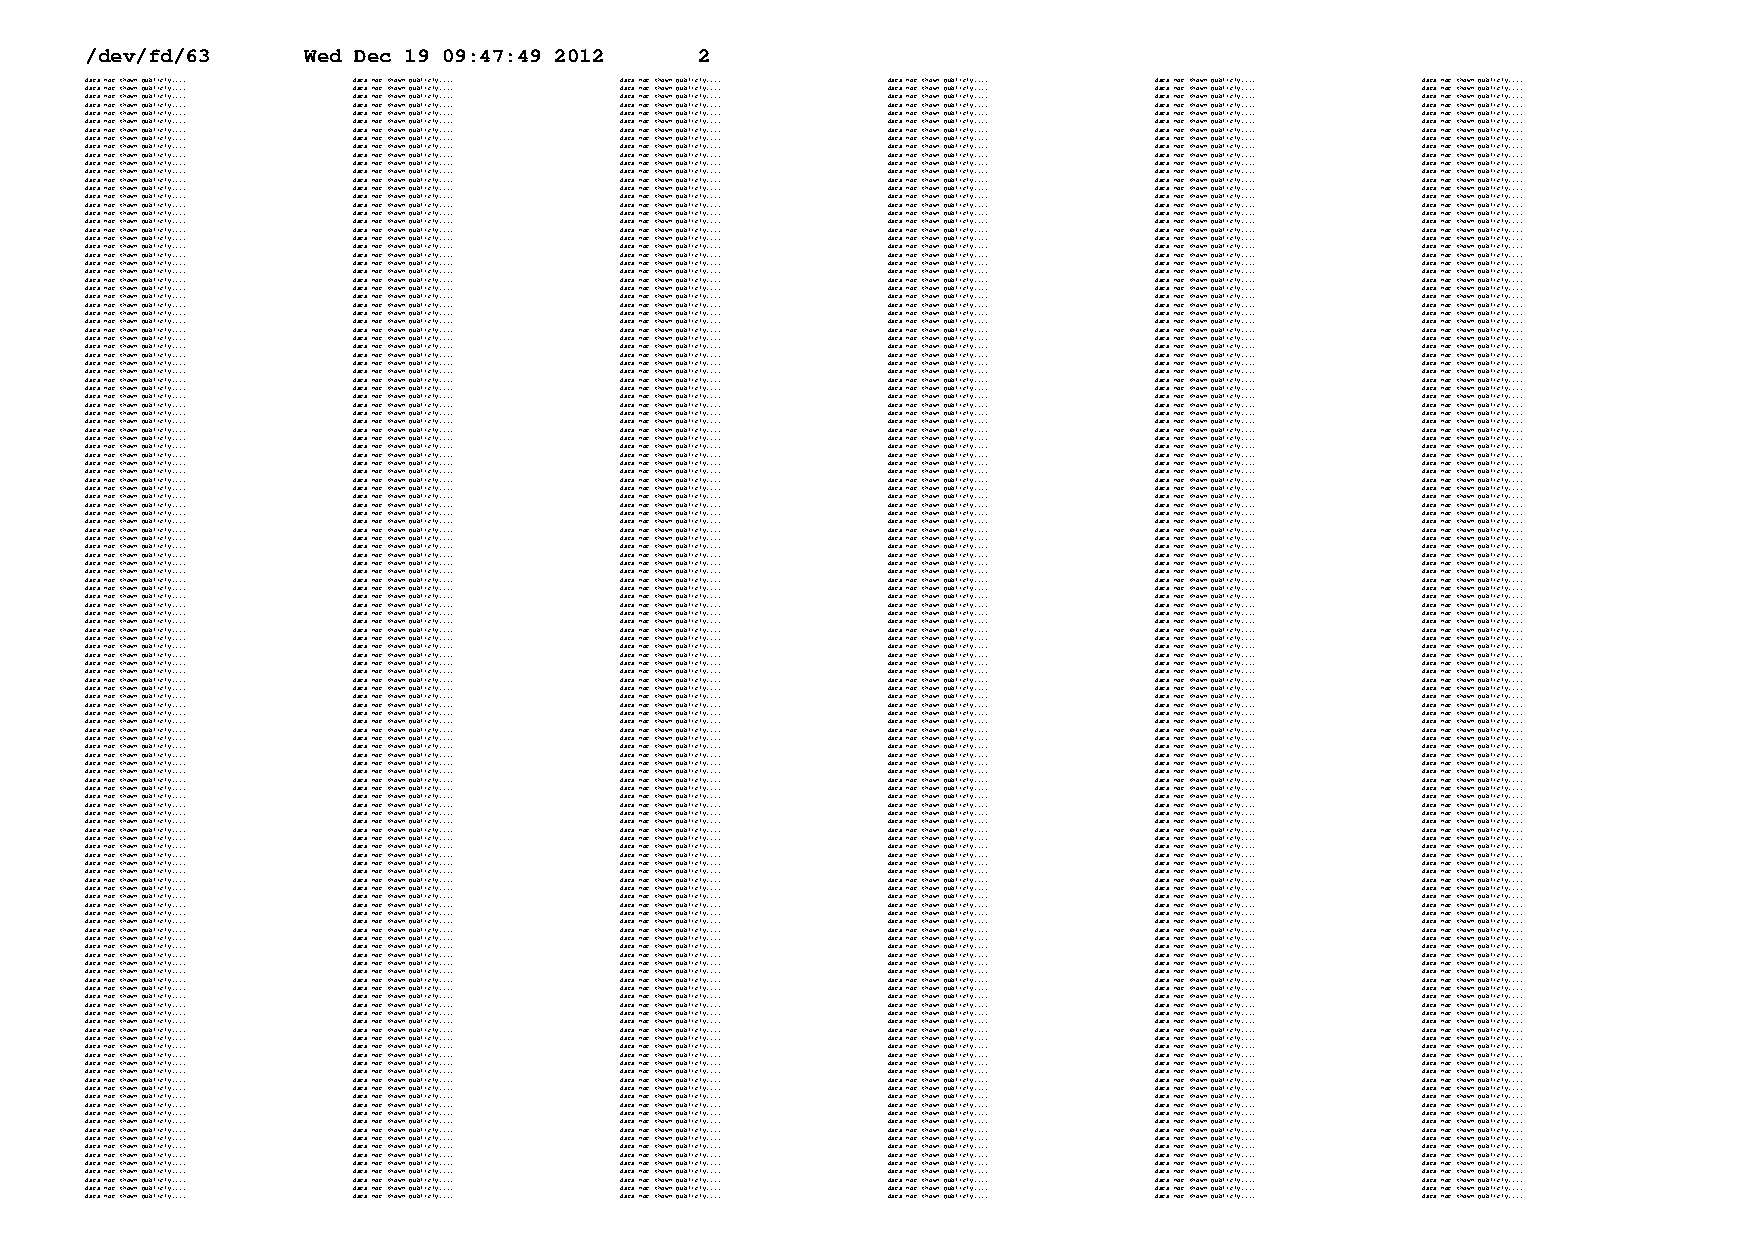
\includegraphics[width=\linewidth]{passwd-page}
\end{frame}

\begin{frame}%
\begin{tikzpicture}[remember picture,overlay]
\fill[black] (current page.north east) rectangle (current page.south west);
\end{tikzpicture}%
\strut
\color{white}
\vfill
\centering
\Huge{Live demonstration}
\vfill
\end{frame}


\newcommand{\cm}[1]{
\structure<+>{#1 \rlap{\onslide<.>{ ?}\onslide<.(1)->{ \checkmark}}}\\
}

\begin{frame}
\frametitle{Did our promise hold?}

Haskell is indeed 
\begin{center}
\Large
\cm{functional}
\cm{pure}
\cm{lazy evaluated}
\cm{strongly typed}
\cm{interpreted}
\cm{compiled}
\end{center}
programming language \ldots

\raggedleft
and it is \alert{fun} to program in.\visible<+- >{ ?}

\end{frame}

\begin{frame}
\frametitle{What we skipped today}
\begin{block}{All the small things\ldots}
\begin{itemize}
\item More about data types
\item (Many) more benefits from the type system
\item Polymorphism
\item Type classes
\item Monads
\item Foreign Function Interface
\end{itemize}
\end{block}
\pause
\begin{block}{\ldots you will find here}
\begin{itemize}
\item Tutorial “Learn you a Haskell”
\item O’Reilly book “Real World Haskell”
\item Tutorial “Write Yourself a Scheme in 48 Hours”
\end{itemize}
\end{block}
\end{frame}

\begin{frame}
\frametitle{Conclusion}
\begin{block}{Writing Haskell code}
\begin{itemize}
\item takes less time,
\item produces less bugs and
\item is more fun.
\end{itemize}
\end{block}
\vfill
Therefore, CU all on 
\begin{center}
\structure{\#haskell} on IRC (freenode)
\end{center}
and on the 
\begin{center}
\structure{haskell-cafe}@haskell.org mailing list!
\end{center}
\end{frame}

\begin{frame}%
\begin{tikzpicture}[remember picture,overlay]
\fill[black] (current page.north east) rectangle (current page.south west);
\end{tikzpicture}%
\strut
\color{white}
\vfill
\small{© 2012 Joachim Breitner.\\
Distributed under the terms of the Creative Commons Attribution license.}
\end{frame}

\end{document}

